\section{Running other people's programs}\label{sec:box}

This section is the argument of the release. It has three parts: why a daily machine must run programs it cannot vouch for, how a capability microkernel turns a short signed list into enforcement, and what we saw when we tried to get past it.

\subsection{Why the machine has to}

The case for refusing everything we did not sign is easy to make and hard to live with. A machine that runs only the project's own capsules can be proved, in the sense of Section~\ref{sec:chain}, down to the byte. It also has no password manager the person has used for years, no Telegram, no \code{git}, no Monero command-line wallet and no way to open a PDF that arrived by email. People route around a machine like that. They keep the real work on another computer, which is the computer the proofs were meant to protect them from.

So the machine has to run programs written by others, and the ones people want are not small. KeePassXC 2.7.8 is a Qt~5 application. Telegram Desktop 5.0.1 is Qt~6 with 254 packages in its install. Neither will be rewritten as a capsule. The honest options are to run them as they are, or not to run them.

Running them as they are raises a second question that most systems answer badly: what does the program get? On a typical desktop, a program started by the person has the person's authority. It can read their files, signal their other programs, open any socket and start any tool. The permission model, where there is one, is a set of dialogs answered by someone who cannot see what is behind them. A Linux password manager that wants the network and a Linux image viewer that wants the network are indistinguishable at the prompt.

\nonos{} makes a different trade. A program gets a box, the box is a short list fixed in advance and signed with the program's Marketplace listing, and anything not on the list is refused with a message that says why. The person decides before install, by reading the list, not at runtime, by guessing.

\subsection{Why a capability microkernel fits}

Holding a program to a list is an old idea, and the usual trouble is where the check lives. In a monolithic kernel the check is a patchwork of hooks on the paths a program might take, and a missed path is a hole. A capability microkernel starts from the other side. A process has nothing unless it holds a capability, and almost every service a program could want is a message to a named capsule that has its own capability word.

That structure gives the box three properties, and they are the reason the design is built the way it is.

First, the guest holds nothing. A Linux program is a process created with an empty capability word. The kernel installs the word with \code{install\_spawn(pid, 0)} and logs \code{[FOREIGN] guest pid=... caps=...} with the mask read back, so the log states what the guest holds instead of assuming it.\src{src/process/foreign/spawn_guest.rs:41-48} With no bits, every native call a guest could make fails the cap table. The one exception is \code{MkTtyQuery}, which only describes the caller's own streams.\src{src/syscall/contract/cap_table/mk_surface.rs:56-60} A guest that learns \nonos{}'s system-call numbers gains nothing, because it has no token that admits them.

Second, every other call goes to one place. A Linux system call number is a small integer, and \nonos{} native numbers are four ASCII letters, so the kernel does not recognise a Linux call. It parks the guest thread and wakes the capsule that created it, its supervisor.\src{src/process/foreign/trap.rs:28-57} The supervisor is \code{capsule\_linux}, the personality. It is the only capsule that holds \code{ForeignExec}, and the kernel lets it touch only the guests it made: the peer calls that map, copy, protect and unmap guest memory begin with \code{supervised\_asid}, which refuses any pid the caller does not supervise.\srcs{src/process/foreign/peer_guard.rs:64-73}{docs/security/capsule-isolation-the-linux-personalitys.md} One supervisor holds at most 1,024 guests and threads.\src{src/process/foreign/room.rs:33-37} So there is no path from a guest to the world that does not pass through the personality, and the kernel, not the personality, guarantees it.

Third, the checker is itself a capsule. It is signed, enrolled under the policy root and admitted by the STARK gate like any other, and it holds a fixed capability word. If the checker has a bug, the damage is bounded by that word, which Section~\ref{sec:capsules} listed. This is weaker than it sounds and stronger than the alternative. It is weaker because the word includes \code{FileSystem} and \code{Crypto}. It is stronger because the checker is a small ring-3 program with a published word, not a patchwork inside the kernel.

Figure~\ref{fig:box} draws the path of one call.

\begin{figure}[t]
\centering
\begin{tikzpicture}[
  font=\small,
  box/.style={draw=ink,line width=0.6pt,rounded corners=2pt,align=center,inner sep=5pt,minimum height=1.35cm,fill=white},
  ring0/.style={box,fill=paper},
  note/.style={font=\footnotesize,text=mute,align=center},
  arr/.style={-{Stealth[length=5pt]},line width=0.6pt,draw=ink},
  darr/.style={-{Stealth[length=5pt]},line width=0.6pt,draw=teal,dashed}]
\node[box,text width=2.5cm] (g) {\textbf{Linux program}\\[2pt]\footnotesize \hbox{empty capability} word};
\node[ring0,text width=3.0cm,right=1.2cm of g] (k) {\textbf{Kernel, ring 0}\\[2pt]\footnotesize no Linux number is native: park the guest, wake its supervisor};
\node[box,text width=3.5cm,right=1.2cm of k] (p) {\textbf{capsule\_linux}\\[2pt]\footnotesize mask, call set, the 17 calls refused on purpose, file world};
\node[box,text width=2.5cm,right=1.0cm of p] (n) {\textbf{Network instance}\\[2pt]\footnotesize holds \code{Network} only if the box has \code{NET\_ANON}};
\draw[arr] (g) -- node[above,note]{syscall} (k);
\draw[arr] (k) -- node[above,note]{frame} (p);
\draw[arr] (p) -- node[above,note]{stream} (n);
\draw[arr] ([xshift=-0.6cm]p.south) -- ++(0,-0.6) -| node[pos=0.25,above,note]{answer} ([xshift=0.6cm]k.south);
\node[ring0,text width=6.2cm,below=1.5cm of k,xshift=1.6cm] (h) {\textbf{Kernel's own record}\\[2pt]\footnotesize every call and its answer, counted in 513 buckets, refused or not};
\draw[darr] ([xshift=-0.6cm]k.south) -- ++(0,-0.75) -| ([xshift=-1.6cm]h.north);
\node[note,above=0.15cm of p] {evaluates the box};
\node[note,above=0.15cm of g] {holds nothing};
\node[note,below=0.2cm of h] {Solid: the path of the call. Dashed: the count the kernel keeps.};
\end{tikzpicture}

\caption{What happens to one Linux system call from a program in a box. The kernel parks the call and hands it to the one supervisor; the supervisor checks the call against the program's policy; the kernel counts the call and the answer in its own record. The program's native capability word is empty. Sources: \code{src/process/foreign/trap.rs}, \code{userland/capsule\_linux/src/linux/app/}, \code{src/process/foreign/seal/}.}
\label{fig:box}
\end{figure}

A word about what we do not say. It is tempting to write that the kernel checks the box on every call. The code says something more careful. The kernel guarantees that every call reaches the checker and that a guest has no other way out. The box itself, the mask and the declared call set, is evaluated by \code{capsule\_linux}. The kernel also keeps a record of its own: it counts every call and its answer into 513 buckets, split into refused and not refused, as the answer is posted, so the record and the answer cannot part.\srcs{src/process/foreign/seal/hist.rs:16-49}{src/process/foreign/seal/absorb.rs:30-38} The two work together. The personality refuses a call outside the declared set with \code{EPERM}, which lands on the refused side of the kernel's count, so a record of a run can show that the box held without trusting what the personality says about itself.\src{userland/capsule_linux/src/linux/app/calls.rs:16-56} Whether that record is checked end to end on a booted release is a separate question, and Section~\ref{sec:box-limits} answers it.

\begin{figure}[t]
\centering
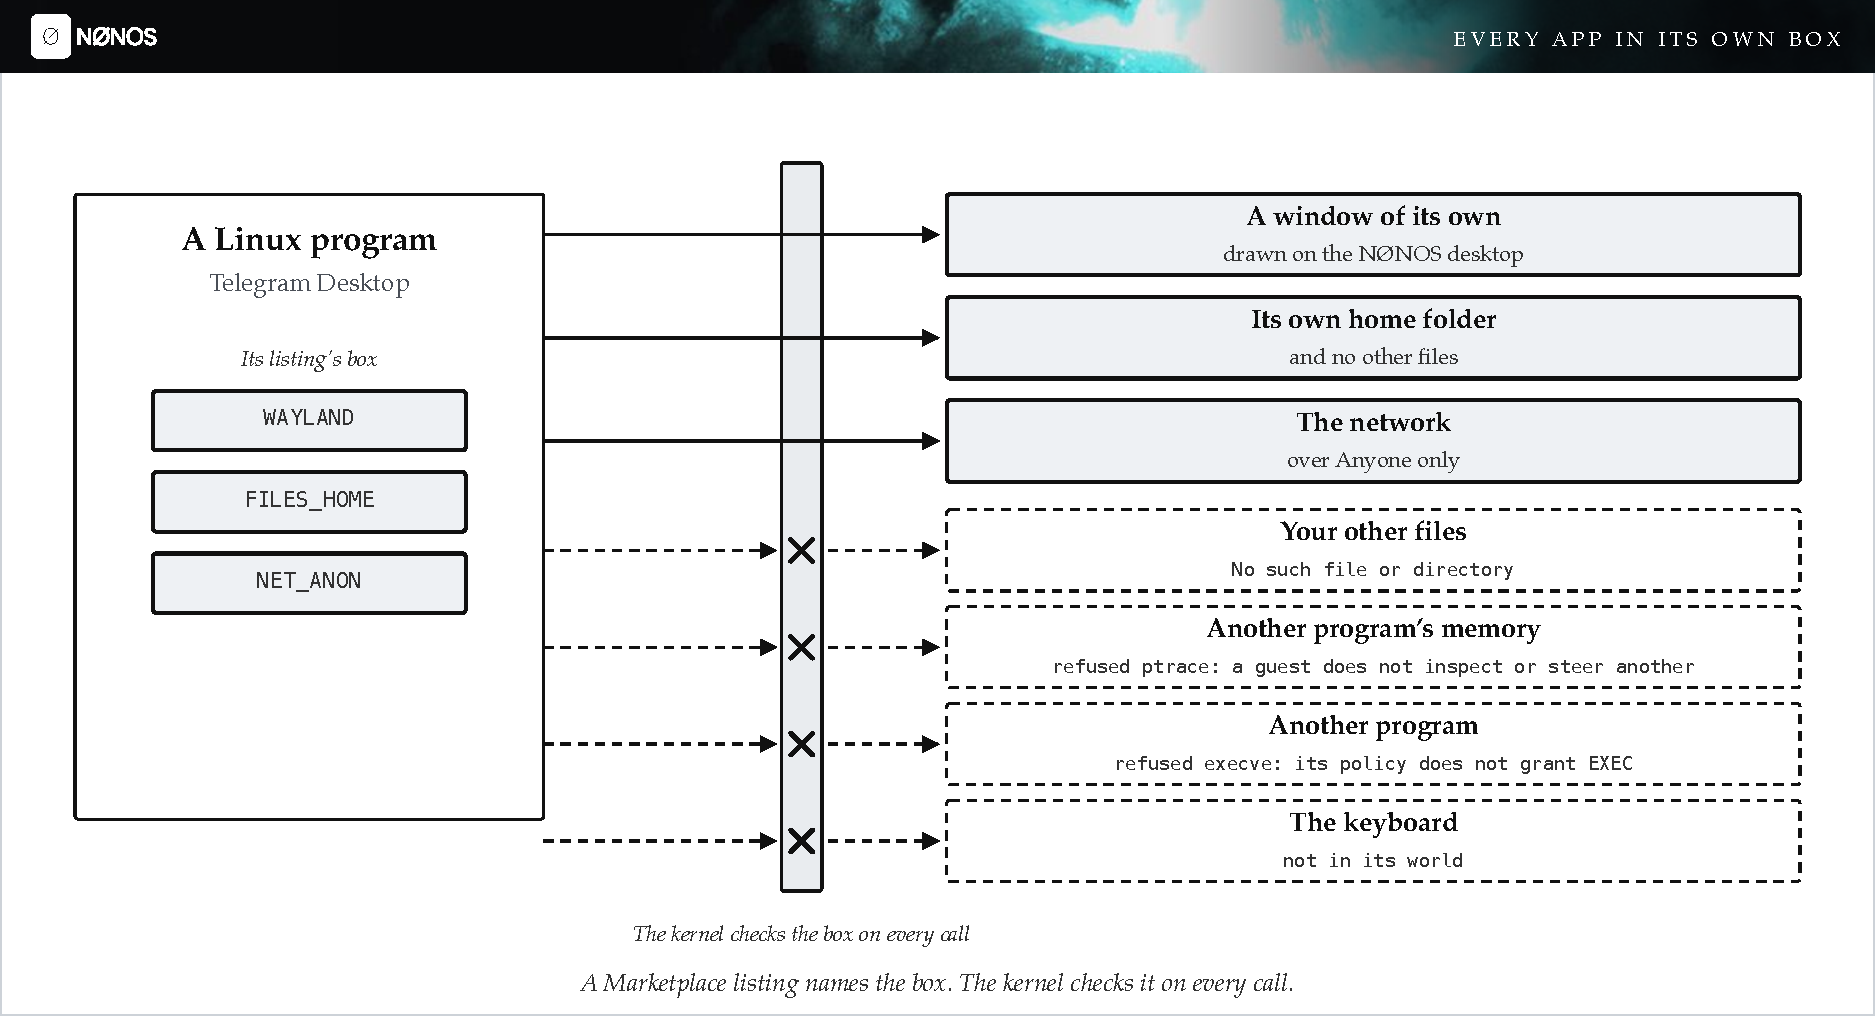
\includegraphics[width=0.84\textwidth]{figures/diagram-the-box.pdf}
\caption{What a program in a box reaches, drawn for Telegram Desktop, whose listing grants \code{WAYLAND}, \code{FILES\_HOME} and \code{NET\_ANON}. Solid arrows are granted, dashed ones are refused, with the answer shown. The band's phrase, "the kernel checks the box on every call", is the project's; the text above and Figure~\ref{fig:box} say how the checking is divided between the kernel and the personality. \code{NET\_ANON} reaches the network the person chose, over Nym or Anyone, never Direct. Sources: \code{docs/using/linux-box.md}, \code{docs/using/marketplace.md}.}
\label{fig:thebox}
\end{figure}

\subsection{What a box is}

A box is 256 bytes. The layout is fixed: the magic \code{NLXPOL01}, a version, the BLAKE3 of the program, a mask of ten service bits, the listing and release ids, a hash of the destination list, and a bit for each of 512 Linux system-call numbers with one more for the native bucket. The decoder accepts exactly the bytes the encoder writes and refuses a wrong length, a non-zero reserved byte, a mask bit with no meaning, or a call bit past bucket 512, so a policy has one encoding and so one hash.\srcs{userland/nonos_linux_policy/src/layout.rs:16-38}{userland/nonos_linux_policy/README.md:1-20} That hash is what a release signs. The \emph{app id}, a BLAKE3 over the program's hash and the policy's hash, is what the personality notes in the kernel's record, so a proof names the program and its box together and neither can be swapped under the other.\src{userland/nonos_linux_policy/src/identity.rs:16-40}

The ten mask bits are the whole vocabulary. Table~\ref{tab:bits} gives them with the number of the 31 catalogue programs that hold each.

\begin{table}[t]
\centering
\caption{The words a box is written in, and how many of the \nPrograms{} Marketplace programs hold each. Three further words exist in the code: \code{FILES\_USER} (the person's own files), \code{MODELS\_RO} (reading the local models) and \code{SERVE\_ONE} (one listener at a port a policy names); the catalogue generator refuses a recipe that asks for \code{FILES\_USER}, so no listed program has it. Counted from \code{userland/capsule\_market/linux-catalogue.json}; definitions in \code{userland/nonos\_linux\_policy/src/mask.rs}.}
\label{tab:bits}
% generated by paper/tools/gen_tables.py from linux-catalogue.json
\begin{tabular}{@{}llr@{}}
\toprule Box word & What it lets the program have & Programs\\ \midrule
\texttt{WAYLAND} & a window of its own on the desktop & 7\\
\texttt{TTY} & the Terminal & 24\\
\texttt{FILES\_HOME} & its own home folder, and no other files & 31\\
\texttt{EXEC} & starting other programs, each held to the same box & 8\\
\texttt{NET\_ANON} & outbound streams, over Nym or Anyone only & 8\\
\texttt{NET\_LISTEN\_LO} & listening on the machine's own loopback & 3\\
\texttt{JIT} & making code as it runs & 1\\
\bottomrule
\end{tabular}

\end{table}

\begin{description}[leftmargin=0pt,style=unboxed,font=\normalfont\code,itemsep=0.3em]
\item[WAYLAND] A window of its own on the desktop, and the input routed to it. Without it, a program that opens the display socket gets \code{EACCES} and the personality logs \code{refused the display: its policy does not grant WAYLAND}.\src{userland/capsule_linux/src/linux/unix/sock.rs:35-37}
\item[FILES\_HOME] Its own home folder. A guest's \code{/} is a tree in the file store, not the person's file system; \code{/home} and \code{/root} are private to the run and kept in memory; without the word they are the shared tree's, read and never written.\note{\path{userland/capsule_linux/src/linux/file/private/rule.rs:16-40}; \path{docs/userland/linux-personality.md}, section "The filesystem a guest sees".}
\item[NET\_ANON] Outbound streams, through the library that applies the person's chosen route, over Nym or Anyone and never Direct, even when Direct is the default network.\srcs{userland/nonos_linux_policy/src/mask.rs:22-26}{userland/capsule_linux/src/linux/net/guest_route.rs:59-75}
\item[EXEC] Starting other programs. Each program started is held to no more than the program that started it, so a chain of \code{execve} cannot widen the box.\src{userland/nonos_linux_policy/src/mask.rs:63-70}
\item[TTY, NET\_LISTEN\_LO, JIT] The terminal; listening on loopback inside the program's own family; making code as it runs.
\end{description}

A program that arrives with no policy at all gets a default box: the terminal, its own home and \code{EXEC}, every call allowed, no window and no network.\src{userland/nonos_linux_policy/src/unlisted.rs:16-40} The comment in the code calls this a project decision, and says that changing it is changing one constant. It is generous on purpose, so command-line tools keep working. It is also the box on the screenshot in Figure~\ref{fig:refusals}, because the programs run there were typed at the Terminal and have no listing.

\subsection{From a listing to a running program}

A listing is where the box is written down. A Marketplace listing for a Linux program carries the Alpine package, a pin of the package's BLAKE3, the program's licence, and a \code{guest\_policy}: the 256 bytes above, written for the exact program the installer will record. The listing's release is signed by its publisher and the index by the Marketplace operator. A schema-3 Linux release with no policy answers \emph{Missing} and can never be installed.\srcs{docs/userland/marketplace-catalogue.md}{userland/capsule_linux/src/linux/install/market/run.rs:34-62}

An install goes through the six gates in Table~\ref{tab:gates}, then fetches the package and what it needs one package at a time over the chosen route, checks each against the Alpine index the catalogue pins, and records the program whose bytes the policy names. A policy the market does not vouch for refuses the install. A failure names the package and the check that stopped it, for example \code{libzmq-4.3.5-r2 (its checksum did not match the signed index)}.\note{\path{docs/using/marketplace.md}, section "How a listing is checked before it installs"; \path{docs/release/0.9.3-what-is-new.md}, section "Installing Linux apps".}

\begin{table}[t]
\centering
\caption{The six gates a Marketplace release must pass before an install is queued. The window decides nothing on its own: it queues a request, and the kernel asks the market for its verdict again. Source: \code{docs/using/marketplace.md}.}
\label{tab:gates}
\begin{tabular}{@{}l>{\raggedright\arraybackslash}p{10.6cm}@{}}
\toprule Gate & Passes when\\ \midrule
index signature & the operator's signature over the catalogue verifies\\
package present & the release names a package URL, a package hash and a manifest hash\\
publisher signature & the release's publisher signature verifies\\
operator validation & the operator marked the release validated\\
architecture & the release runs on \code{x86\_64-nonos} or \code{x86\_64-linux} and needs kernel ABI 1 at most\\
attestation & the release carries a proof trailer hash, or it is a \code{linux.} listing, whose proof this machine makes after it has checked the bytes\\ \bottomrule
\end{tabular}
\end{table}

\begin{figure}[t]
\centering
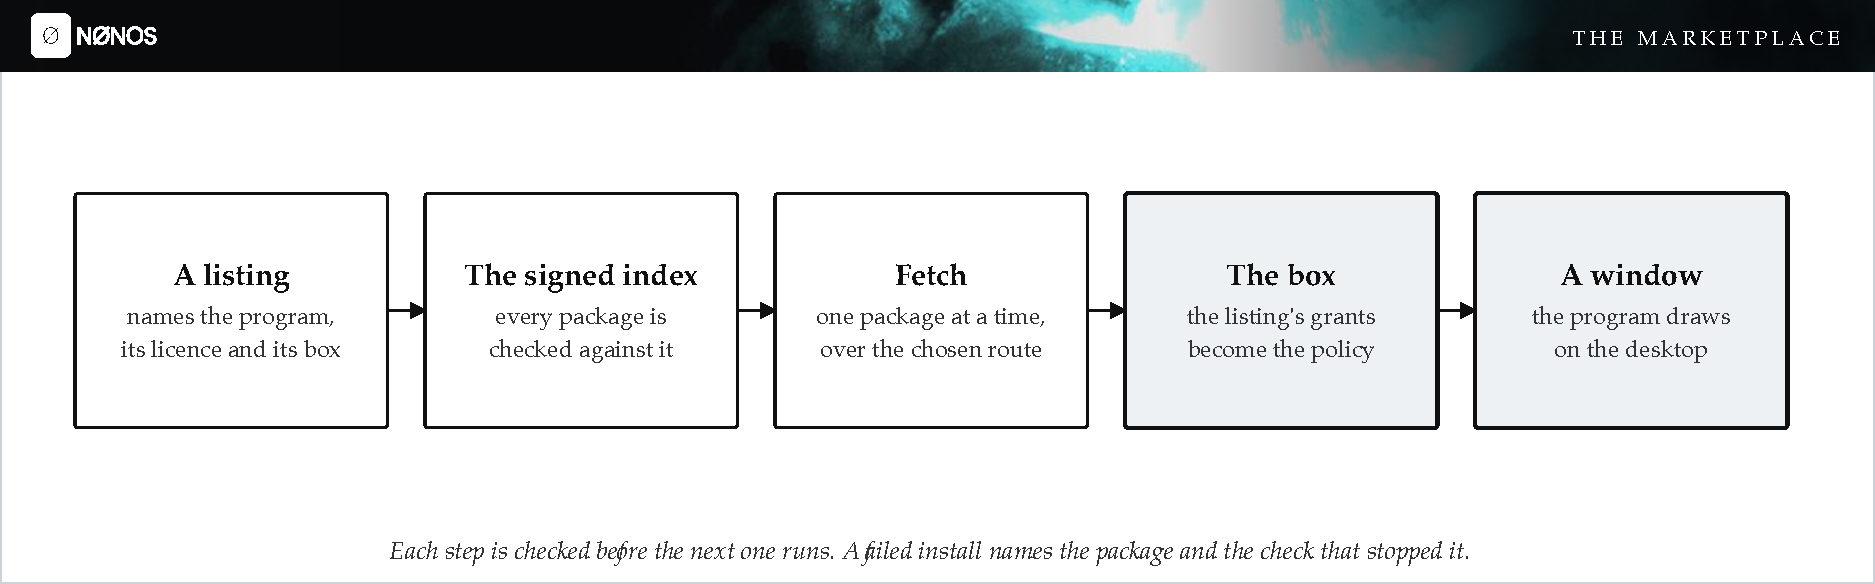
\includegraphics[width=0.84\textwidth]{figures/diagram-install-and-run.pdf}
\caption{From a listing to a window. A listing names the program, its licence and its box; the package is checked against the signed index; the install fetches one package at a time over the chosen route; the listing's grants become the policy; the program draws a window. A failed install names the package and the check that stopped it. Sources: \code{docs/userland/marketplace-catalogue.md}, \code{docs/using/marketplace.md}.}
\label{fig:install}
\end{figure}

The weakest word in that account is "proof". The attestation gate for a Linux listing says that the machine makes the proof itself after checking the bytes. That is the local-authority path of Section~\ref{sec:capsules}, a keyed tag, not a vendor STARK. What the person gets is a chain of checks on identity: the Alpine index signature, the catalogue's pin, the operator's and publisher's signatures, the bytes. The STARK stays with the project's own capsules.\note{\path{docs/using/marketplace.md}, section "How a listing is checked before it installs".} We want the distinction to be plain, because it is the one a reader is most likely to blur. The proof is about \nonos{}'s capsules, and the box is about everyone else's programs.

\subsection{Enforcement, one layer at a time}

The box is enforced in three places, and each does a different job.

\textbf{The kernel's part} is the structure above: an empty word for the guest, one supervisor, peer access only to a supervisor's own guests, a count of every call. It does not know what a Linux call means. The record is explicit that it counts numbers only.

\textbf{The personality's part} is the box itself, and it is done call by call. Before a call is served, a bucket the policy leaves clear is \code{EPERM}, except \code{exit} and \code{exit\_group}, which are served whatever the set says.\srcs{userland/capsule_linux/src/linux/app/rules.rs:21-31}{userland/capsule_linux/src/linux/app/calls.rs:36-56} Beyond that, the personality holds a short list of calls it refuses on purpose with a stated reason: seventeen of them, among them \code{ptrace}, \code{process\_vm\_readv}, \code{process\_vm\_writev}, \code{mount}, \code{chroot}, \code{unshare}, \code{setns} and \code{io\_uring}, which is refused as "a second call path around the gate".\src{userland/capsule_linux/src/linux/serve/refused.rs:21-47} A guest sees only its own processes in \code{/proc}, has no input devices, and cannot name the person's files because they are not in its world.\srcs{docs/release-evidence/0.9.3/s1-isolation-61ec29ea2/README.md}{README.md} An internet socket needs one of \code{NET\_ANON}, \code{NET\_LISTEN\_LO} or \code{SERVE\_ONE}; \code{execve} needs \code{EXEC}.\srcs{userland/capsule_linux/src/linux/net/socket.rs:30-47}{userland/capsule_linux/src/linux/call/spawn/exec.rs:28-31}

\textbf{The network is enforced twice.} The personality never holds \code{Network} in its ordinary run and terminal roles. A program whose box includes \code{NET\_ANON} is started again in a different instance of the personality, \code{app.linux.run.net} or \code{app.linux.term.net}, which does hold the \code{Network} bit, and which exits unless the policy it binds grants \code{NET\_ANON}. A box without \code{NET\_ANON} never runs there; the network role refuses it.\srcs{src/userspace/capsule_linux/run_net.rs:16-34}{src/userspace/capsule_linux/role_term_net.rs:22-44}\src{userland/capsule_linux/src/linux/app/rules.rs:42-61} So for a program without the network word there are two independent refusals: the personality will not make an internet socket, and the instance serving it holds no capability with which the kernel would carry one. That second refusal is the kernel's, and it does not depend on the personality being right.

\subsection{Windows}

The new part of 0.9.3 that a person sees is that a Linux program opens its own window on the \nonos{} desktop. The personality serves a Wayland display to a guest whose box grants \code{WAYLAND}. The guest speaks the Wayland wire protocol over a Unix socket the personality implements: registry, \code{wl\_shm} buffers, \code{xdg} toplevels, seats and keymaps, data devices, output, decoration. The window is registered as a surface with the compositor through the two graphics bits the personality holds, and drawn inside the toolkit's own frame, with a \nonos{} title bar and close, minimise and maximise buttons.\srcs{userland/capsule_linux/src/linux/wayland/mod.rs:19-60}{docs/release-evidence/0.9.3/gui-frame/README.md} A surface's frame callbacks are answered at most 30 times a second, and at once for an idle window.\src{userland/capsule_linux/src/linux/wayland/pace_rule.rs:17-28}

The window is the cheapest thing in the box to give and the most delicate. A guest that holds \code{WAYLAND} can draw anything inside its own window and receive input routed to it. Whether one Linux window can reach another program's surface is a question we have not tested, and it is on the list of things we have not attacked.

What has been shown to run is narrower than the catalogue. On development images, swayimg drew its window, zoomed and closed; its frame's close button ended it with status 0; foot drew its window and ran a shell over \code{/dev/pts}; KeePassXC 2.7.8 drew its welcome screen in a box of \code{WAYLAND} and \code{FILES\_HOME}, once the personality served \code{FUTEX\_WAKE\_OP}, which Qt~5 uses to wake a waiting thread. On a KVM run of the release tree, Telegram Desktop installed from the real Alpine mirror over Anyone and drew its welcome screen. No sign-in or sent message was shown. mpv and zathura are listed and no boot in the evidence shows a window for either. DarkFi's chat app is listed and no boot shows its window. Mousepad is not listed, because on the release tree it started in its box and showed no window.\note{\path{docs/release/0.9.3-what-is-new.md}, section "Linux programs in their own windows"; \path{docs/release/0.9.3-known-issues.md}, section "Linux windows".}

Dragging a Linux window by its title bar and minimising it are not shown. Copy and paste between a Linux window and the desktop is tested on the host only.\note{\path{docs/release/0.9.3-known-issues.md}, section "Linux windows".}

\begin{figure}[t]
\centering
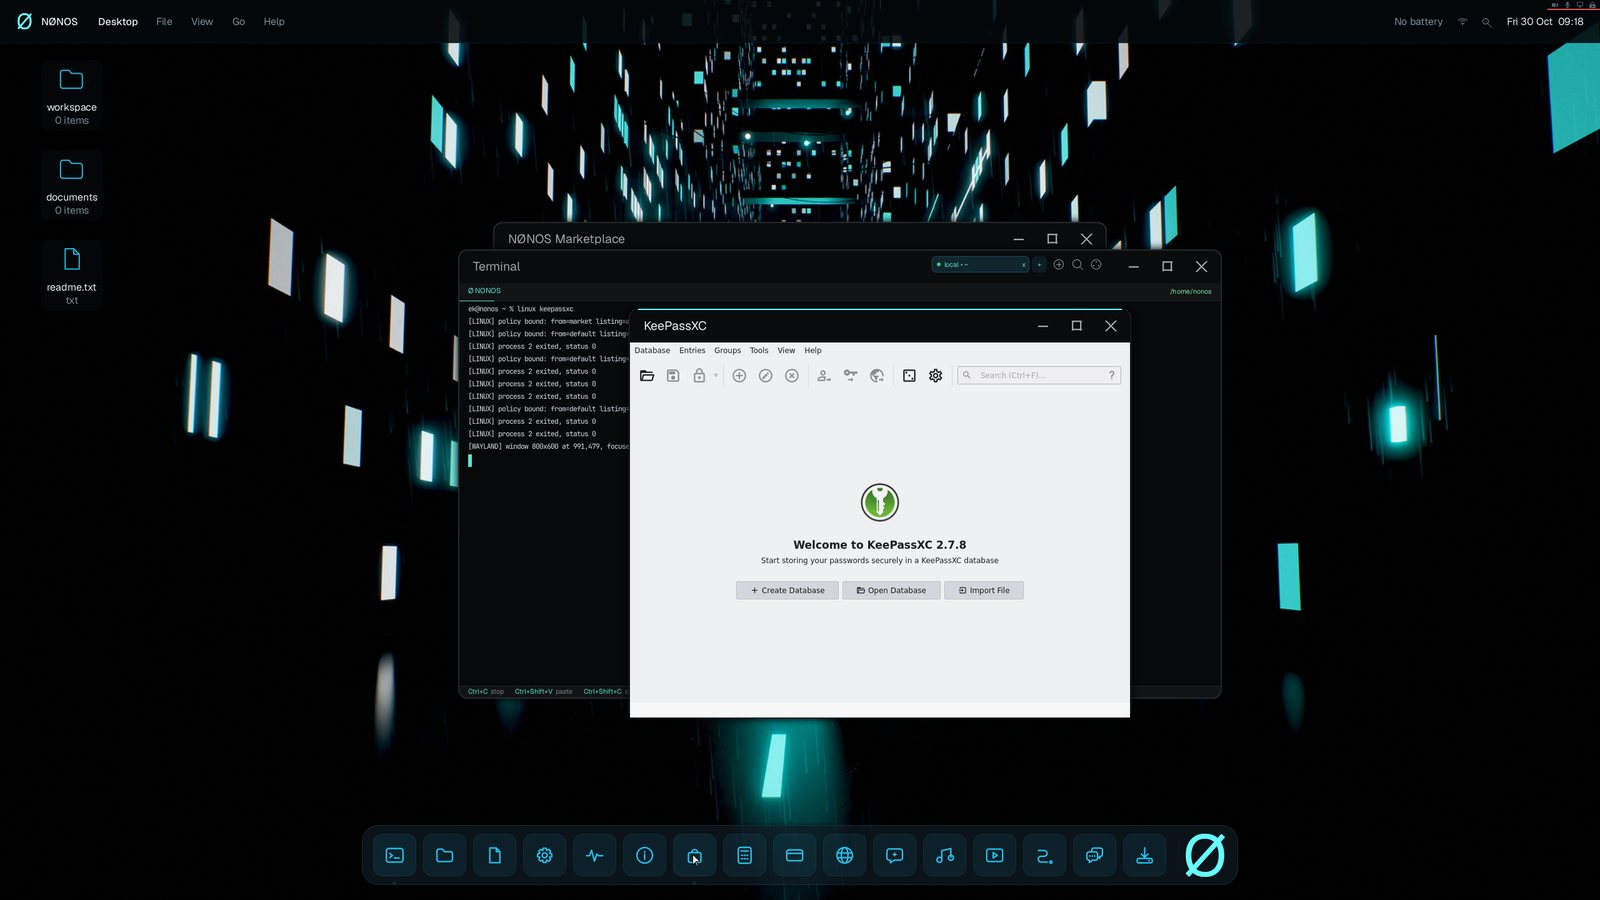
\includegraphics[width=0.82\textwidth]{figures/keepassxc-in-its-box.jpg}
\caption{KeePassXC 2.7.8, a Linux password manager, drawing its own window on the \nonos{} desktop, with the Terminal that started it behind it showing \code{[LINUX] policy bound} lines. Its box is \code{WAYLAND} and \code{FILES\_HOME}: a window and a home folder, no network. Sealed 0.9.3 image under KVM. The screenshot shows a welcome screen; it does not show a database being made or opened.}
\label{fig:keepass}
\end{figure}

\subsection{Terminals}

A terminal emulator opens a pseudo-terminal before it starts a shell, and until 0.9.3 there was none to open. A guest can now open \code{/dev/ptmx}, and \code{/dev/pts/N} opens the slave once it is unlocked. A family holds at most 64 pairs. What the master writes passes the slave's line discipline: input mapping, \code{\string^C} as a signal for the foreground group under \code{ISIG}, line editing under \code{ICANON}, echo. A changed window size raises \code{SIGWINCH}. When the master goes, the slave reads end of file and its session leader gets \code{SIGHUP}.\note{\path{docs/userland/linux-personality.md}, section "Pseudo-terminals"; \path{userland/capsule_linux/src/linux/pty/table.rs:25-50}.} A master writing with no reader stops at 4,096 pending bytes or lines and 64~KiB of output.\note{\path{docs/release/0.9.3-what-is-new.md}, section "Pseudo-terminals".} foot ran a shell over \code{/dev/pts} on a development image. That is the one booted use we can point to.\src{docs/release-evidence/0.9.3/gui-foot/README.md}

\subsection{The thirty-one programs}

Table~\ref{tab:programs} lists the catalogue as it stands in the tree: 31 entries, each with its box and licence. One of them, the SimpleX Chat core, is an engine for a window that is not in this release and is not meant to be run directly, so 30 are things a person starts. The release notes count 30 recipes for that reason, and the README counts 31 rows.\note{\path{userland/capsule_market/linux-catalogue.json}; \path{docs/release/0.9.3-what-is-new.md}, section "The Marketplace".}

Two features of the table are worth reading before the table. First, every program holds \code{FILES\_HOME}, and no program holds the person's files: the box for a text editor is a terminal and its own empty home. Second, only eight programs hold \code{NET\_ANON}, and the ones that do are chat clients, wallets and Telegram. The shipped listings name no destinations, so a program with \code{NET\_ANON} may open a stream to any host and port over the chosen route. A destination list is part of the policy format, and \code{linux --box} accepts one, but the catalogue uses it for none of its entries.\src{userland/capsule_market/linux-catalogue.json}

\begin{table}[t]
\centering
\caption{The \nPrograms{} programs in the Marketplace catalogue with their boxes, grouped by what they draw. Generated from \code{userland/capsule\_market/linux-catalogue.json} by \code{paper/tools/gen\_tables.py}. Twenty-five come from Alpine v3.20 packages. The other six are not Alpine packages: DarkFi's four are built from source at a pinned commit, and SimpleX's two are the upstream release binary pinned by hash. A listing in this table is not evidence that the program has run: the status of each is in Section~\ref{sec:status}.}
\label{tab:programs}
% generated by paper/tools/gen_tables.py from linux-catalogue.json
{\footnotesize\setlength{\tabcolsep}{4pt}
\begin{longtable}{@{}>{\raggedright\arraybackslash}p{3.6cm}>{\raggedright\arraybackslash}p{6.6cm}>{\raggedright\arraybackslash}p{4.2cm}@{}}
\toprule Program & Its box & Licence\\ \midrule\endhead
\multicolumn{3}{@{}l}{\textit{With a window of their own} (7)}\\
swayimg & \texttt{WAYLAND FILES\_HOME} & MIT\\
Telegram Desktop & \texttt{WAYLAND FILES\_HOME NET\_ANON} & GPL-3.0-or-later + exc.\\
KeePassXC & \texttt{WAYLAND FILES\_HOME} & GPL-2.0-only OR GPL-3.0-only\\
foot (terminal) & \texttt{WAYLAND TTY FILES\_HOME EXEC} & MIT\\
mpv (media player) & \texttt{WAYLAND FILES\_HOME} & GPL-2.0-or-later\\
zathura (PDF viewer) & \texttt{WAYLAND FILES\_HOME} & Zlib\\
DarkFi (chat app) & \texttt{WAYLAND FILES\_HOME NET\_ANON} & AGPL-3.0-only\\
\addlinespace
\multicolumn{3}{@{}l}{\textit{In the Terminal} (23)}\\
Helix & \texttt{TTY FILES\_HOME} & MPL-2.0\\
micro & \texttt{TTY FILES\_HOME} & MIT\\
Kakoune & \texttt{TTY FILES\_HOME EXEC} & Unlicense\\
Vim & \texttt{TTY FILES\_HOME} & Vim\\
bat & \texttt{TTY FILES\_HOME EXEC} & Apache-2.0\\
eza & \texttt{TTY FILES\_HOME} & MIT\\
nnn & \texttt{TTY FILES\_HOME EXEC} & BSD-2-Clause\\
ncdu & \texttt{TTY FILES\_HOME} & MIT\\
fzf & \texttt{TTY FILES\_HOME EXEC} & MIT\\
Git & \texttt{TTY FILES\_HOME EXEC} & GPL-2.0-only\\
tig & \texttt{TTY FILES\_HOME EXEC} & GPL-2.0-or-later\\
lazygit & \texttt{TTY FILES\_HOME EXEC} & MIT\\
age & \texttt{TTY FILES\_HOME} & BSD-3-Clause\\
minisign & \texttt{TTY FILES\_HOME} & ISC\\
FLAC & \texttt{TTY FILES\_HOME} & BSD-3-Clause AND GPL-2.0-or-later\\
LAME & \texttt{TTY FILES\_HOME} & LGPL-2.0-or-later\\
Geth (dev chain) & \texttt{TTY FILES\_HOME NET\_LISTEN\_LO} & GPL-3.0-or-later\\
Profanity (XMPP, OMEMO) & \texttt{TTY FILES\_HOME NET\_ANON} & GPL-3.0-or-later\\
Monero wallet (CLI) & \texttt{TTY FILES\_HOME NET\_ANON} & BSD-3-Clause\\
DarkFi wallet (drk) & \texttt{TTY FILES\_HOME NET\_ANON} & AGPL-3.0-only\\
DarkFi local dev chain & \texttt{TTY FILES\_HOME NET\_LISTEN\_LO JIT} & AGPL-3.0-only\\
DarkIRC (P2P chat) & \texttt{TTY FILES\_HOME NET\_ANON NET\_LISTEN\_LO} & AGPL-3.0-only AND MIT\\
SimpleX Chat (terminal) & \texttt{TTY FILES\_HOME NET\_ANON} & AGPL-3.0-only\\
\addlinespace
\multicolumn{3}{@{}l}{\textit{A background engine} (1)}\\
SimpleX Chat core & \texttt{FILES\_HOME NET\_ANON} & AGPL-3.0-only\\
\bottomrule
\end{longtable}}

\end{table}

\subsection{What the kernel refused}

We ran Linux programs on the sealed 0.9.3 image under KVM and tried the things a hostile program would try. Figure~\ref{fig:refusals} is the Terminal after three of them, and Table~\ref{tab:refusals} lists six, each with the answer the system gave.

\begin{figure}[t]
\centering
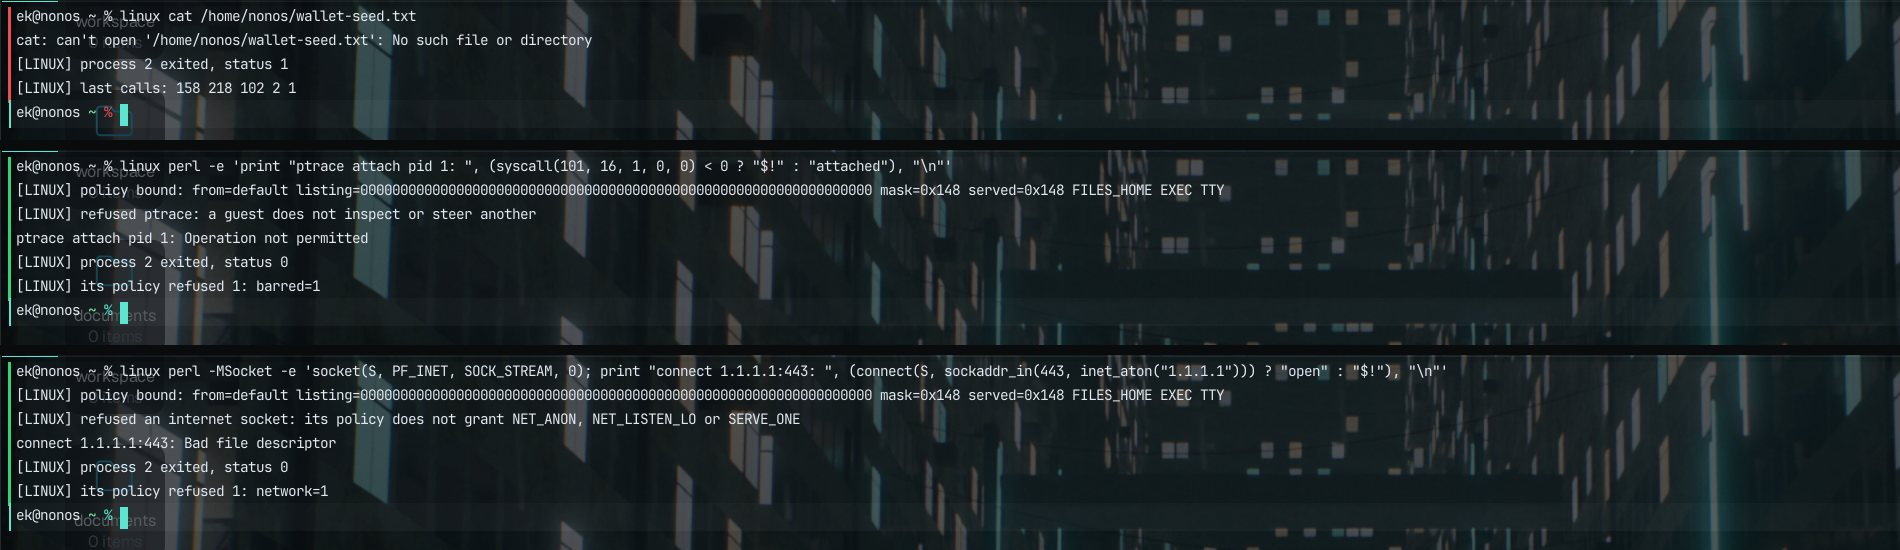
\includegraphics[width=\textwidth]{figures/refusals.jpg}
\caption{The Terminal after three attempts from inside a Linux program: reading a file that is not in its world, attaching with \code{ptrace} to process 1, and opening an internet socket and connecting out. The \code{policy bound} lines show \code{from=default}, a listing of all zeros and \code{mask=0x148}, which is \code{FILES\_HOME}, \code{EXEC} and \code{TTY}: the default box of a program typed at the Terminal with no listing. Sealed 0.9.3 image under KVM, no TPM. Single attempts, as the next paragraph says.}
\label{fig:refusals}
\end{figure}

\begin{table}[t]
\centering
\caption{Six attempts from inside a Linux program on the sealed 0.9.3 image, and what the system answered. The first three are in Figure~\ref{fig:refusals}. The other three come from the project's README table of the same run, whose screenshot we do not have. The fourth, the refused \code{execve}, needs a box without \code{EXEC}, so it was not run in the default box of the figure.}
\label{tab:refusals}
\footnotesize
\begin{tabular}{@{}>{\raggedright\arraybackslash}p{3.3cm}>{\raggedright\arraybackslash}p{11.2cm}@{}}
\toprule Attempt & Answer\\ \midrule
Read the person's files & \code{cat: can't open '/home/nonos/wallet-seed.txt': No such file or directory}; its \code{/home} is empty\\
Attach to another process & \code{[LINUX] refused ptrace: a guest does not inspect or steer another}\\
Open a connection out & \code{[LINUX] refused an internet socket: its policy does not grant NET\_ANON, NET\_LISTEN\_LO or SERVE\_ONE}\\
Start another program & \code{[LINUX] refused execve: its policy does not grant EXEC}\\
See other programs & \code{ls /proc} shows one process, its own\\
Read the keyboard & \code{cat /dev/input/event0}: no such device\\ \bottomrule
\end{tabular}
\end{table}

These are single attempts from inside an app. They are not an exploit chain, and nobody has tried one. A program that is granted a right is allowed it: Telegram's box gives it the network, and it uses the network. We do not claim the box cannot be broken. What the attempts show is narrower and, to us, still worth having: the refusals are specific, they name the missing word, and they come from the code paths in Section~\ref{sec:box} that we can point to.

A second, earlier suite is committed with its serial log. A Perl script on a development image tried what a hostile app would: \code{ptrace} and \code{process\_vm\_readv} on process 1, a kernel module load, \code{kexec}, \code{mount}, an anonymous mapping that is both writable and executable, a one-terabyte mapping, a mapping made executable after the fact, signals to every pid, \code{/proc/kcore} and \code{/dev/mem}, a TCP connect and a UDP send with no network word, a raw socket, and a fork loop. Each was refused or bounded; the fork loop stopped at 511, the family's ceiling. That boot was under QEMU's software emulation, on a branch with one extra system call that this release does not carry, and the first attempt at it was thrown away because Perl's \code{syscall} took the wrong argument.\src{docs/release-evidence/0.9.3/s1-isolation-61ec29ea2/README.md} We include the failed attempt because it is the usual way such a test goes wrong.

The kernel's side of the story is visible in the \code{audit} command, shown in Figure~\ref{fig:audit}. It lists every process with the reach its capability word gives it (network, storage, devices, launch), who signed it and every bit it holds. Kernel threads show as not in the registry, with no signed ceiling recorded.\src{userland/capsule_terminal/src/command/builtin/audit/table.rs:16-66}

\begin{figure}[t]
\centering
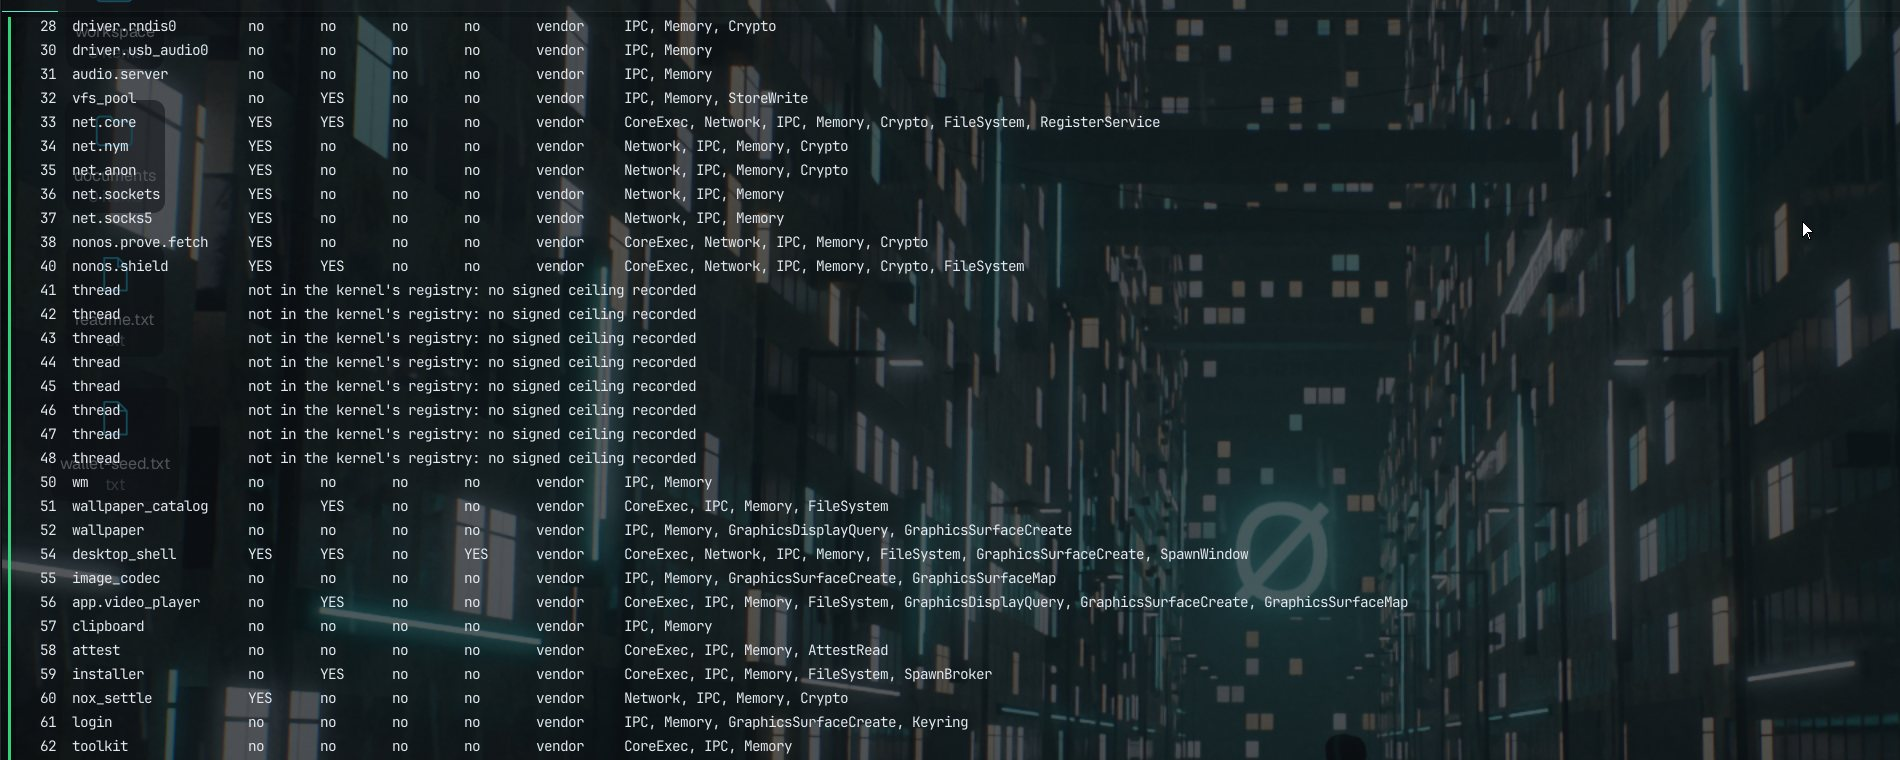
\includegraphics[width=\textwidth]{figures/audit.jpg}
\caption{Part of the \code{audit} table on the sealed 0.9.3 image under KVM. Columns after the name are four reach areas (network, storage, devices, launch), the signer (\code{vendor} for every row shown) and the capability bits the process holds. Rows 41 to 48 are threads, which have no signed ceiling. The \code{devices} column names capability bits the kernel would honour, not devices claimed at the moment.}
\label{fig:audit}
\end{figure}

\subsection{Running a program you wrote, or a model did}

The same machinery is available by hand. \code{linux --box} runs a program in a named box and prints a report of what the box refused:

\begin{verbatim}
linux --box strict sh -c 'echo ok > /tmp/out; echo no > /home/out; nc 10.0.0.1 80'
linux --box offline python3 script.py
linux --box allow:/tmp/out,net:api.example.com:443 python3 agent.py
\end{verbatim}

\code{strict} has no network and writes only to \code{/tmp}. An \code{allow:} box names its folders and, if it needs any, its destinations. A connection anywhere else is refused and counted, and the destination list is the one place in the current tree where a box can name hosts. \code{linux --box learn} runs a program once, enforced as \code{offline}, and writes the tightest box file that would have let it do what it did. The file is one run's behaviour, not what the program may need on another, and the documentation says to read it before use.\src{docs/using/linux-box.md} The report's counts are made by the personality as it refuses; they are not the kernel's histogram, and the page says so. This is the use we expect from people who run code a model wrote: a throwaway box, a printed list of what it tried, a file to tighten next time.

\subsection{Where the box is weak}\label{sec:box-limits}

The box is a design with a working implementation, not a finished wall, and we would rather say where it is thin than wait for someone else to.

\textbf{The call set does not narrow anything yet.} A recipe without a measured set is \emph{unmeasured}: buckets 0 to 511 set and 512 clear, so every Linux call is allowed and only the native bucket is barred. None of the 31 catalogue entries carries a measured set. The machinery to enforce a narrower one exists and is tested on the host, and a listing could use it, but the boxes in Table~\ref{tab:programs} are, in practice, the mask plus the seventeen calls refused on purpose.\note{\path{docs/userland/marketplace-catalogue.md}, section "The recipes file"; \path{userland/nonos_linux_policy/src/market.rs:31-43}.}

\textbf{The box is kept by path.} The catalogue documentation lists three ways around it that are open today: a listed package's dependencies install unheld and run in the default box (tig pulls git, bat pulls less, vim pulls xxd); a held program copied to another path along with its trailer; and the loader invoked as \code{/lib/ld-musl-x86\_64.so.1 <program>}, because the loader's gate checks only the trailer. Each ends in the default box, with every call allowed and no network. The proposed fix, tying a policy to the program's hash and not its path, is not in this release. We rely on that page at this commit; we did not re-run the three.\note{\path{docs/userland/marketplace-catalogue.md}, section "What a listing carries".}

\textbf{The supervisor is a large target.} It holds \code{FileSystem}, \code{Crypto}, \code{StoreWrite}, \code{ForeignExec} and \code{Debug} at all times, and the threat model says that authority follows the process, not the code. A program that takes over the personality gets those bits. One personality instance serves a run's guests together, a program and everything it starts. The personality's own documentation reports 369 host tests passing in the flake checks; the Linux surface is still a large amount of code to hold to a policy.\note{\path{docs/security/protections-and-limits-what-nonos-does.md}; \path{docs/userland/linux-personality.md}, section "Tests".}

\textbf{A home does not survive power-off.} A Linux program's home is held in memory, at most 16~MiB (64~MiB for the Monero wallet) and 128 names, and is gone at power-off. A home kept across a reboot is designed and not in the release, so the only lasting copy of a wallet seed is the one written down.\note{\path{userland/capsule_linux/src/linux/file/system/declared/home.rs:29-32}; \path{docs/release/0.9.3-known-issues.md}, section "Linux apps".} The design page says in its first line that kept homes move to the next release.\src{docs/design/kept-homes-and-installs.md}

\textbf{The proof of a run has not completed on a boot.} The Marketplace's proof of how a program ran timed out in two boots, and the 180-second wait that followed is not booted. Programs also fail in ways the tree states plainly: \code{lame} ended on signal 11 on a development boot, \code{micro} opened from the Marketplace stops on \code{open /dev/tty}, and \code{age}'s passphrase prompt, which writes to \code{/dev/tty}, does not show.\note{\path{docs/release/0.9.3-known-issues.md}, section "Linux apps".}

\textbf{Nobody outside the project has attacked it.} The refusals above were produced by us, against our own code, on images we built. That is not an audit.
